
%% Introduction page
%% =============
%%
%% Introduction page
%% =============
%%
Volcanic activities on Earth have always shaped the Earth surface and influenced atmospheric processes.
Volcanism is a geological phenomenon which is related to the rise of magma from the Earth's interior to the Earth's surface. Volcanic activity is linked to tectonic active regions, thus hotspots mainly are at the margins of the continental plates.
significantly less volcanic activities occur at the interior of continental or oceanic shelves \citep{schmincke2000vulkanismus}.\\
Volcanoes are often particularly recognized by their dramatic consequences of a major volcanic eruption. But volcanoes influence our lives in more than this way. Volcanic gases can have an effect on weather by emitting aerosols or on larger time-scales even the climate \citep{schmidt2015volcanismarticle}. 
Examples are the Laki eruption in Iceland (1783-1784) followed by a very hot summer and a cold winter in central Europa \citep{thordarson2003atmospheric} and the Tambora eruption, Indonesia in 1815 which caused the "year without summer" in 1816.\\
Volcanic gases can alter the radiative balance of the Earth due to scattering and absorption of solar radiation \citep{schmidt2015volcanism}.
A decrease of stratospheric ozone (O$_3$) has been observed after the eruption of  El Chickon in 1982 and the eruption of Mount Pinatubo in 1991. The depletion comes from volcanic aerosols which serve to transform anthropogenic chlorine/bromine into more reactive forms \citep{solomon1998ozone}. 
%
\newline
%
The gas composition of the volcano plume change with activity and can be an indicator for the processes inside the Earth .\\ 
The change of the gas composition with volcanic activity is a result of the specific pressure dependency of the solubility of each dissolved gases within the magma. Therefore the relative concentration of a gas change with its origin source depth due to pressure dependency on the depth below the crater vent. Therefore the ratio of two gases can be used to draw conclusions on the origin source depth of the gases.
%
This work particularly deals with the ratio of BrO and SO$_2$. The advantage of using the ratio of these two gases is the possibility of getting continues data by using the NOVAC spectral data.\\
The BrO to \ce{SO2} ratio changes due to pressure differences with depth, thus the BrO/\ce{SO2} ratio changes with its origin source depth. It is possible to conclude from the BrO/\ce{SO2} ratio to the degassing source depth and therefore the ratio is a proxy for volcanic processes. A change in BrO/\ce{SO2} prior to eruption was observed at Etna and Nevado del Ruiz.\\
%
\newline
%
The Network for Observation of Volcanic and Atmospheric Change (NOVAC) is a network to record volcanic emissions. The aim of NOVAC is mainly to provide new parameters for risk assessment and volcanological research, both locally and on a regional and global scale.
NOVAC is a Network of spectrographic instruments located next to about 30 volcanoes in Asia, America, Africa and Europe. At each of these volcanoes are two to four spectrograph's installed, recording back-scattered solar radiation spectra at different viewing angles.\\
NOVAC is a network which produces a large amount of data and thus provides the chance to evaluate long time periods which is a unique opportunity to study volcanic trace gases.\\
The instruments and the maintenance need to be cheap, thus the instruments need to have a rather simple construction. Therefore it was decided not to implement temperature stabilization even at the expense of the quality of the data.\\
%
\newline
%
The data recorded by NOVAC are evaluated using Differential Optical Absorption Spectroscopy (DOAS) \citet{platt2008differential}. DOAS utilizes the wavelength dependency of the absorption of light and is based on the Beer-Lambert law. The gas concentration is retrieved from the characteristic difference in absorption structures between the plume and a reference region. Thus it is fundamental to have a reference which is free of the gases of interest, to assure that the retrieved concentration is correct.
%
\newline
%
The reference region is usually treated as free of
volcanic trace gases. If the reference region is for any reason
contaminated by volcanic trace gases, the reference spectrum has to be
replaced by a volcanic-gas-free reference. Alternative spectra could be for example a
theoretical solar atlas spectrum or a volcanic-gas-free reference
spectrum recorded in the temporal proximity (eg. a day before) by the same instrument.
The first option comes with the drawback of reduced precision, as the
instrumental effects have to be modeled and added to the retrieval. The reduction in precision is acceptable for the \ce{SO2} retrieval, but not suitable for a BrO retrieval because then most data would be below the detection limit. The advantage of the first option is, that the absolute column density is calculated, since, the theoretical solar atlas spectrum is absolutely gas free. For the second option, the alternative reference spectrum should
have been recorded at similar conditions with respect to meteorology,
radiation, intensity and in temporal proximity due to instrumental changes
with time and ambient conditions. We combined both options in order to
achieve both, enhanced accuracy but still maximum possible precision of
the \ce{SO2} and BrO retrievals. We present an algorithm which finds the
optimal reference spectrum automatically. As first step, a possible \ce{SO2}
contamination of the standard reference is checked by a comparison with
the theoretical solar atlas. If a contamination is detected, as second step,
the algorithm picks a volcanic-gas-free reference (beforehand
automatically checked for contamination) from another scan.\\
%
\newline
%
To gain a better understanding volcanism it is elementary to improve the measurement techniques. The aim of this thesis is to improve the retrieval of the BrO/SO2 ratio by using data from Tungurahua in Ecuador and Nevado del Ruiz a volcano located in Colombia, provided by NOVAC.



%%%%%%%%%%%%%%%%%
%%%%%%%%%%%%%%%
%%%%%%%%%%%%%%
%%%%%%%%%%%%
















%
%
%
%
%
%\textbf{	warum sind volkane interessant}
%Volcanic activities on Earth have always shaped the Earth  surface and influenced atmospheric processes. Volcanoes are often particularly recognized by their dramatic consequences of a major volcanic eruption. But volcanoes influence our lives in more than this way. Volcanic gases can effect the weather by emitting aerosols  or on larger time-scales even the climate \citet{schmidt2015volcanismarticle}.
%Examples are the Laki eruption in Iceland (1783-1784) followed by a very hot summer and a cold winter in central Europa \citet{thordarson2003atmospheric} and the Tambora eruption, Indonesia in 1815 which caused the "year without summer" in 1816.\\
%\textbf{wie kann man mehr über sie erfahren}
%Volcanism is a geological phenomena which is related to the raise of magma  from the Earth's  interior to the Earth's  surface. Volcanic activity is linked to tectonic active regions, thus hotspots mainly are at the margins of the continental plates.
%significantly less volcanic activities occurs at the the interior of continental or oceanic shelves \citet{schmincke2000vulkanismus}.
%
%The most abundant volatile species released during a volcanic eruption are water vapour (H$_2$O; relative amount of the plume: 50\%-90\%) and carbon dioxide (CO$_2$; relative amount of the plume: 1\%-40\%) \citet{platt2015quantification}. 
%
%But the short time effects of those two gases are rather small since their effect on atmospheric composition is negligibly due to the high abundance of atmospheric H$_2$O and CO$_2$. 
%On higher timescales (100000 years) the volcanic emissions are relevant for preservation of carbon dioxide. 
%
%But on timescales of the age of the Earth  the volcanic emission of H$_2$O and CO$_2$ largely contributed on the formation of our Atmosphere \citet{schmidt2015volcanism}.\\ 
%
%A typically volcanic plume consists of many different gases alongside H$_2$O and CO$_2$  sulfur dioxide (SO$_2$) contributes with 1\%-25\% to the plume, hydrogen sulfide (H$_2$S) with 1\%-10\% and hydrogen chloride with (HCl) 1\%-10\%. Furthermore there are trace gases for example carbon disulfide (CS$_2$), carbon sulfide (COS) carbon monoxide (CO) hydrogen fluoride (HF), hydrogen bromide (HBr) and many other species \citet{platt2015quantification}.\\
%%
%A decrease of stratospheric ozone (O$_3$) has been observed after the eruption of  El Chickon in 1982 and the eruption of Mount Pinatubo 1991. The depletion comes from volcanic aerosols which serve to transform anthropogenic chlorine/bromine into more reactive forms \citet{solomon1998ozone}. 
%%
%Volcanic gases can alter the radiative balance of the Earth  due to scatter and absorption of solar radiation \citet{schmidt2015volcanism}.\\
%
%Volcanoes emit various gases in the atmosphere. This can occur due to volcanic eruptions or due quiet degassing. Gas emitted by quiet degassing remains in the troposphere while eruptions can inject volcanic gases up to the stratosphere \citet{robock2000volcanic}. The larger lifetime in the stratosphere and a larger sensitivity of the stratospheric chemistry to volcanic gases leads to an higher impact on the earth climate of these gases.
%Volcanic gases have a large influence on the earth climate especially \ce{CO2} and \ce{SO2}  or more specific its oxidation product sulfur acid.\\ 
%The relevance of  \ce{CO2} for the climate is a subject of many discussions about the climate change. Compared to other atmospheric \ce{CO2} sources, the share of volcanic  \ce{CO2} is rather low.\\
%\\
%Even though the \ce{SO2} emissions during eruptive episodes are up to one order higher than during quite degassing episodes, \citet{halmer2002annual} estimates that quiescent degassing contributes 40\% of the accumulated \ce{SO2} between 1972 to 2000.\\
%\citet{halmer2002annual} estimated the mean annual \ce{SO2}  emitted from volcanoes from 1972 to 200 as 7.5 to 10.5TgSyr$^{-1}$, while the anthropogenic \ce{SO2}  amount for 2000 is estimated as 55 TgSyr$^{-1}$ \citep{IPCC}. Despite the less \ce{SO2}  occurring from volcanoes the impact may be higher as the impact of the anthropogenic \ce{SO2}. \citet{graf1997volcanic} supposed that the volcanic \ce{SO2}  has a higher impact on the climate since its reaches up to the stratosphere while the anthropogenic \ce{SO2}  is mostly located in planetary boundary layer. In the lower troposphere sulphuric acid has a lifetime of about a week whereas the lifetime in the stratosphere is about a year \citep{IPCC}.\\
%Sulphuric acid in the atmosphere increases the earth albedo due to direct backscattering radiation. Additional the condensation on sulphuric acid particles leads to finer droplets and thus to more stable and more white clouds. This increases the albedo as well \citep{twomey1974pollution}.
%Volcanic particles can be surfaces for heterogeneous reaction. The result is a depletion of stratospheric ozone, and thus a more high energetic solar flux on the earth surface.
%Large particles may backscatter IR radiation from the earth surface and the lower atmosphere, leading to a small reduction of the net cooling of the lower troposphere.
%In the upper troposphere or stratosphere absorption of IR or UV radiation results in a net heating in the stratosphere and a cooling at the earth surface.
%
%\begin{figure}
%	\centering
%	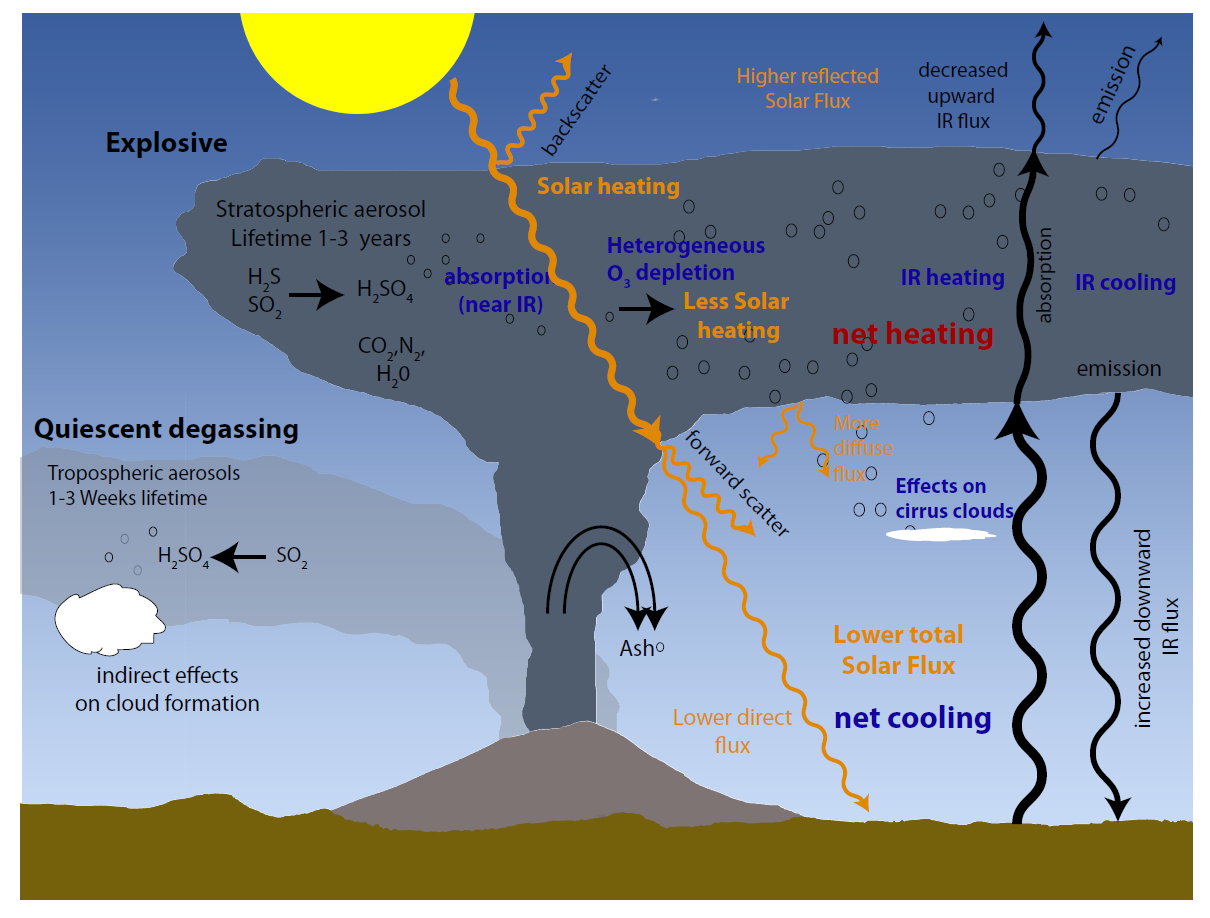
\includegraphics[width=0.8\linewidth]{Bilder/Simon/Bilder_Tung/Climate_Influence}
%	\caption{Influence of volcanic eruptions and quiet degassing on earth climate. Redrawn on the basis of \citet{robock2000volcanic}}
%	\label{fig:climateinfluence}
%\end{figure}
%
%
%\Cref{fig:climateinfluence} shows the above described effects and their localization in the atmosphere.
%The dominating radiative effect of volcanic gases is a cooling of the earth atmosphere due to  more backscattered radiation, more diffusive scattering\citep{robock2000volcanic}.
%\citet{IPCC} records a volcanic radiative forcing of $-0.11W/m^{2}$ between 2008 and 2011. For comparison the radiative of  \ce{CO2} is estimated as  $1.68W/m^{2}$.
%
%%
%The gas composition of the volcano plume change with activity and can be a indicator for the processes inside the Earth .\\ 
%\textbf{wie wird gemessen}
%\textbf{was für daten hat man dann}
%The Network for Observation of Volcanic and Atmospheric Change (NOVAC) is a network to record volcanic emissions. The aim of NOVAC is mainly to provide new parameters for risk assessment and volcanological research, both locally and on a regional and global scale.
%NOVAC is a Network of spectrographic instruments located next to about 30 volcanoes in Asia, America, Africa and Europe. At each of these volcanoes are two to four spectrograph's installed, recording back-scattered solar radiation spectra at different viewing angles.\\
%NOVAC is a network which produces a large amount of data and thus provides the chance to evaluate long time periods which is a unique opportunity to study volcanic trace gases.\\
%The instruments and the maintenance need to be cheap, thus the instruments need to have a rather simple construction. Therefore it was decided not to implement temperature stabilization even at the expense of the quality of the data.\\This thesis utlises NOVAC-data from Tungurahua and Nevado del Ruiz.\\
%%
%The data recorded by NOVAC are evaluated using Differential Optical Absorption Spectroscopy (DOAS) \citet{platt2008differential}. DOAS utilises the wavelength dependency of the absorption of light and is based on the Beer-Lambert law. The gas concentration is retrieved from the characteristic difference in absorption structures between the plume and a reference region. Thus it is fundamental to have a reference which is free of the gases of interest, to assure that the retrieved concentration is correct.
%\textbf{was kann man daraus lernen}
%In this work \textcolor{yellow}{we} are particularly interested in the ratio of BrO and SO$_2$.\textcolor{red}{das muss bessere begründet werden. Warum diese beiden gase? warum nicht Co2? etc}
%
%The BrO to \ce{SO2} ratio changes due to pressure differences with depth, thus the BrO/\ce{SO2} ratio changes with its origin source depth. It is possible to conclude from the BrO/\ce{SO2} ratio to the degassing source depth and therefore the ratio is a proxy for volcanic processes. A change in BrO/\ce{SO2} prior to eruption was observed at Etna and Nevado del Ruiz.\\
%\textbf{was für Probleme treten auf}
%The reference region, is usually treated as free of
%volcanic trace gases. If the reference region is for any reason
%contaminated by volcanic trace gases, the reference spectrum has to be
%replaced by a volcanic-gas-free reference. Alternative spectra could be for example a
%theoretical solar atlas spectrum or a volcanic-gas-free reference
%spectrum recorded in the temporal proximity (eg. a day before) by the same instrument.
%The first option comes with the drawback of reduced precision, as the
%instrumental effects have to be modelled and added to the retrieval. The reduction in precision is acceptable for the \ce{SO2} retrieval, but not suitable for a BrO retrieval because then most data would be below the detection limit. The advantage of the first option is, that the absolute column density is calculated, since, the theoretical solar atlas spectrum is absolutely gas free. For the second option, the alternative reference spectrum should
%have been recorded at similar conditions with respect to meteorology,
%radiation,intensity and in temporal proximity due to instrumental changes
%with time and ambient conditions. We combined both options in order to
%achieve both, enhanced accuracy but still maximum possible precision of
%the \ce{SO2} and BrO retrievals. We present an algorithm which finds the
%optimal reference spectrum automatically. As first step, a possible \ce{SO2}
%contamination of the standard reference is checked by a comparison with
%the theoretical solar atlas. If a contamination is detected, as second step,
%the algorithm picks a volcanic-gas-free reference (beforehand
%automatically checked for contamination) from another scan.\\
%\textbf{ was sin die strategien}
%\textbf{ was macht diese arbeit}
%%
%In this work mainly uses data from Tungurahua in Ecuador and Nevado del Ruiz a volcano located in Colombia.